\section{Auswahl der Daten}
\subsection{Reineke-Gleichung und Mortalitätsrate}
\begin{frame}[c]
  \visible<\theFirstElement->{
    \centerline{
      \(\log(N) = \textcolor{red}{s} \log(D) + k\)
    }
    
    \begin{minipage}{1.0\textwidth}
      \centerline{
        \mycaption{Gleichung: Bestandesdichte in Abhängigkeit von mittlerem Durchmesser (Quelle: [1]).}
      }
    \end{minipage}
    \begin{align*}
      \myscalebox{N} & \myscalebox{: \text{Bestandesdichte [ha\textsuperscript{-1}]}} \\[-3mm]
      \myscalebox{s} & \myscalebox{: \text{Steigung (}\widehat{=}\text{ \textcolor{red}{Mortalitätsrate})}} \\[-3mm]
      \myscalebox{D} & \myscalebox{: \text{Durchmesser des Grundflächemittelstammes [cm]}} \\[-3mm]
      \myscalebox{k} & \myscalebox{: \text{Konstante (artabhängig)}} \\[-3mm]
    \end{align*}}
  
  \begin{itemize}
  \item<\theSecondElement-> Literatur: \\
    Mortalitätsrate scheint art- und standortabhängig zu sein (s. z.B. [2])
  \item<\theSecondElement-> Lösungsansatz: \\
    artabhängiger Korridor ,,erlaubter`` Mortalitätsraten, begrenzt durch unteren Schwellwert (\(m_u\)) und oberen Schwellwert (\(m_o\))
  \end{itemize}
\end{frame}

\subsection{Auswahl-Mechanismus}
\begin{frame}[c]
  \begin{columns}
    \begin{column}{0.5\textwidth}
      \visible<\theFirstElement->{
        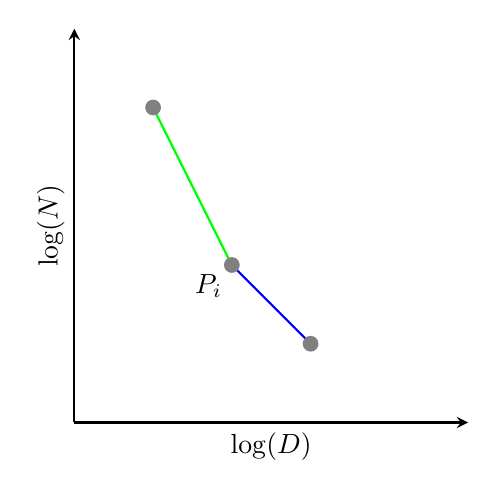
\begin{tikzpicture}[>=stealth]
          %% Coordinate system.
          \draw[black,thick,->] (0,0) -- (5,0);  %% x-axis
          \draw[black,thick,->] (0,0) -- (0,5);  %% y-axis
          \node[anchor=north] at (2.5,0) {\(\log(D)\)};  %% x-axis title
          \node[anchor=south,rotate=90] at (0,2.5) {\(\log(N)\)};  %% y-axis title
          
          %% Specify point coordinates.
          \coordinate (Pi-1) at (1,4);
          \coordinate (Pi) at (2,2);
          \coordinate (Pi+1) at (3,1);

          %% Lines.
          \visible<\theSecondElement->{\draw[green,thick] (Pi-1) -- (Pi);}
          \visible<\theThirdElement->{\draw[blue,thick] (Pi) -- (Pi+1);}

          %% Points.
          \fill[gray] (Pi-1) circle (0.1);
          \fill[gray] (Pi) circle (0.1);
          \fill[gray] (Pi+1) circle (0.1);

          %% Text.
          \node[anchor=north east] at (Pi) {\(\text{P}_i\)};
        \end{tikzpicture}
      }
    \end{column}
    \begin{column}{0.5\textwidth}
      \visible<\theFirstElement->{\(\text{P}_i\) wird ausgewählt, wenn}
      \begin{enumerate}
      \item<\theFirstElement-> es mind. einen benachbarten Punkt gibt und
      \item<\theSecondElement-> Steigung \(\textcolor{green}{s_1} \geq m_u\) und
      \item<\theThirdElement-> Steigung \(\textcolor{blue}{s_2} \leq m_o\).
      \end{enumerate}
    \end{column}
  \end{columns}
\end{frame}

\subsection{Beispiel: Buche}
\begin{frame}[c]
  \visible<1->{
    \centerline{
      \begin{minipage}{0.9\textwidth}
        \includegraphics[width=1.0\textwidth]{../../Graphics/Presentation/logDlogNPlotsBeforeAfterDataSelectionBeech.pdf} \\
        \mycaption{Abbildung: Auswirkung des Auswahl-Mechanismus am Beispiel des Buchen-Datensatzes. Farbige Linien verbinden Beobachtungen eines Bestandes. \\
        A: vor Anwendung des Auswahl-Mechanismus \\
        B: nach Anwendung des Auswahl-Mechanismus }
      \end{minipage}}}
\end{frame}

%%% Local Variables:
%%% mode: latex
%%% TeX-master: "MasArPresentation.tex"
%%% End:
